\chapter{Progress}
\section{Research}
In the first year of my PhD candidature, I mainly focus on the SSE scheme supporting private and efficient query. I and my supervising team design this new SSE scheme named HXT together. The new scheme is based on the `OXT' protocol \cite{cash2013highly}, but its security is further improved by removing a result pattern leakage that leaks the matching pairs of queried keywords. To achieve this, we design a new Hidden Vector Encryption (HVE) scheme without pairing to improve the performance of HVE significantly, and we embedded the new HVE with OXT to hide the result pattern leakage.

Currently the implementation of this scheme in a distributed environment is finished and a comparable dataset with `OXT' is tested in HXT. The result shows that by adopting the in-memory distributed computing framework and distributed database (Spark \cite{apache2017spark} and HBase \cite{apache2017hbase}), the new scheme can also perform efficient queries over encrypted database and the overhead of our HVE is almost negligible because it is only use symmetric encryption primitives. 

The paper of HXT is writing in progress, we will test the HXT protocol in a larger dataset as a supplementary result for its efficiency in large scale database. We plan to submit this paper to IEEE S\&P by 1st Dec.

HXT is a more secure SSE protocol that support boolean query functions, and it is also indexed by inverted index. Hence, HXT can serve as a building block of my Searchable Graph Encryption by providing secure and efficient boolean query functions.

\section{Courseworks}
To meet the coursework requirements, I've get exemption for one compulsory module and attend another one as well as the compulsory events and workshops in FIT 5144 in the first year. However, there are some issues with my grades in FIT6021 module ``Modelling and Computer Simulation''. Table \ref{tlb:coursework} shows the detailed information about my coursework activities. 

\begin{table}[h]
\centering
\begin{tabular}{|c|c|c|}
\hline
\bf Course Code & \bf Course Name & \bf Result \\ \hline
\bf FIT5143 & \bf IT Research Methods & \bf Exempted \\ \hline
\bf  FIT6021 & \bf Advanced Research Methods & \bf C \\ \hline
& Argument Analysis & HD \\ \hline
& Problem Solving and Proof & D \\ \hline
& Scientific Method & HD \\ \hline
& Modelling and Computer Simulation & Attended but Missing \\ \hline
& Design Research & D \\ \hline
\bf FIT5144 & \bf MGE Monash Graduate Research & \bf 4 hours \\ 
& \bf Student Induction &  \\ \hline
\bf FIT5144 & \bf MGE  Research Integrity & \bf 12 hours \\ \hline
\bf FIT5144 & \bf Faculty of IT Induction & \bf 6 hours \\ \hline
\bf FIT5144 & \bf Communicating Research & \bf 30 hours\\ \hline
& Strategies and Plans & completed \\ \hline
& Academic Audiences & completed \\ \hline
& Funding Applications & completed \\ \hline
& Community Audiences & completed \\ \hline
& Lay Audiences & completed \\ \hline
\bf FIT5144 & \bf Ethical Research and Publications & \bf 6 hours\\ \hline
& Philosophical Approaches of Ethic & completed \\ \hline
& Ethic in Publication and Authorship & completed \\ \hline
\end{tabular}
\caption{Coursework Activties and Claimed Hours}
\label{tlb:coursework}
\end{table}

Apart from the compulsory 58 hours' events and workshops listed above, I also attend GSAS Oral Presentations Workshops, Preparing for Confirmation Workshops; The Data61 reading group; Dean's Seminar Series; Staff Appointment Seminar in FIT as elective activities to fulfil the requirement of 120 hours activities attending record for FIT5144.


\chapter{Timeline to Completion}
\begin{figure}[h]
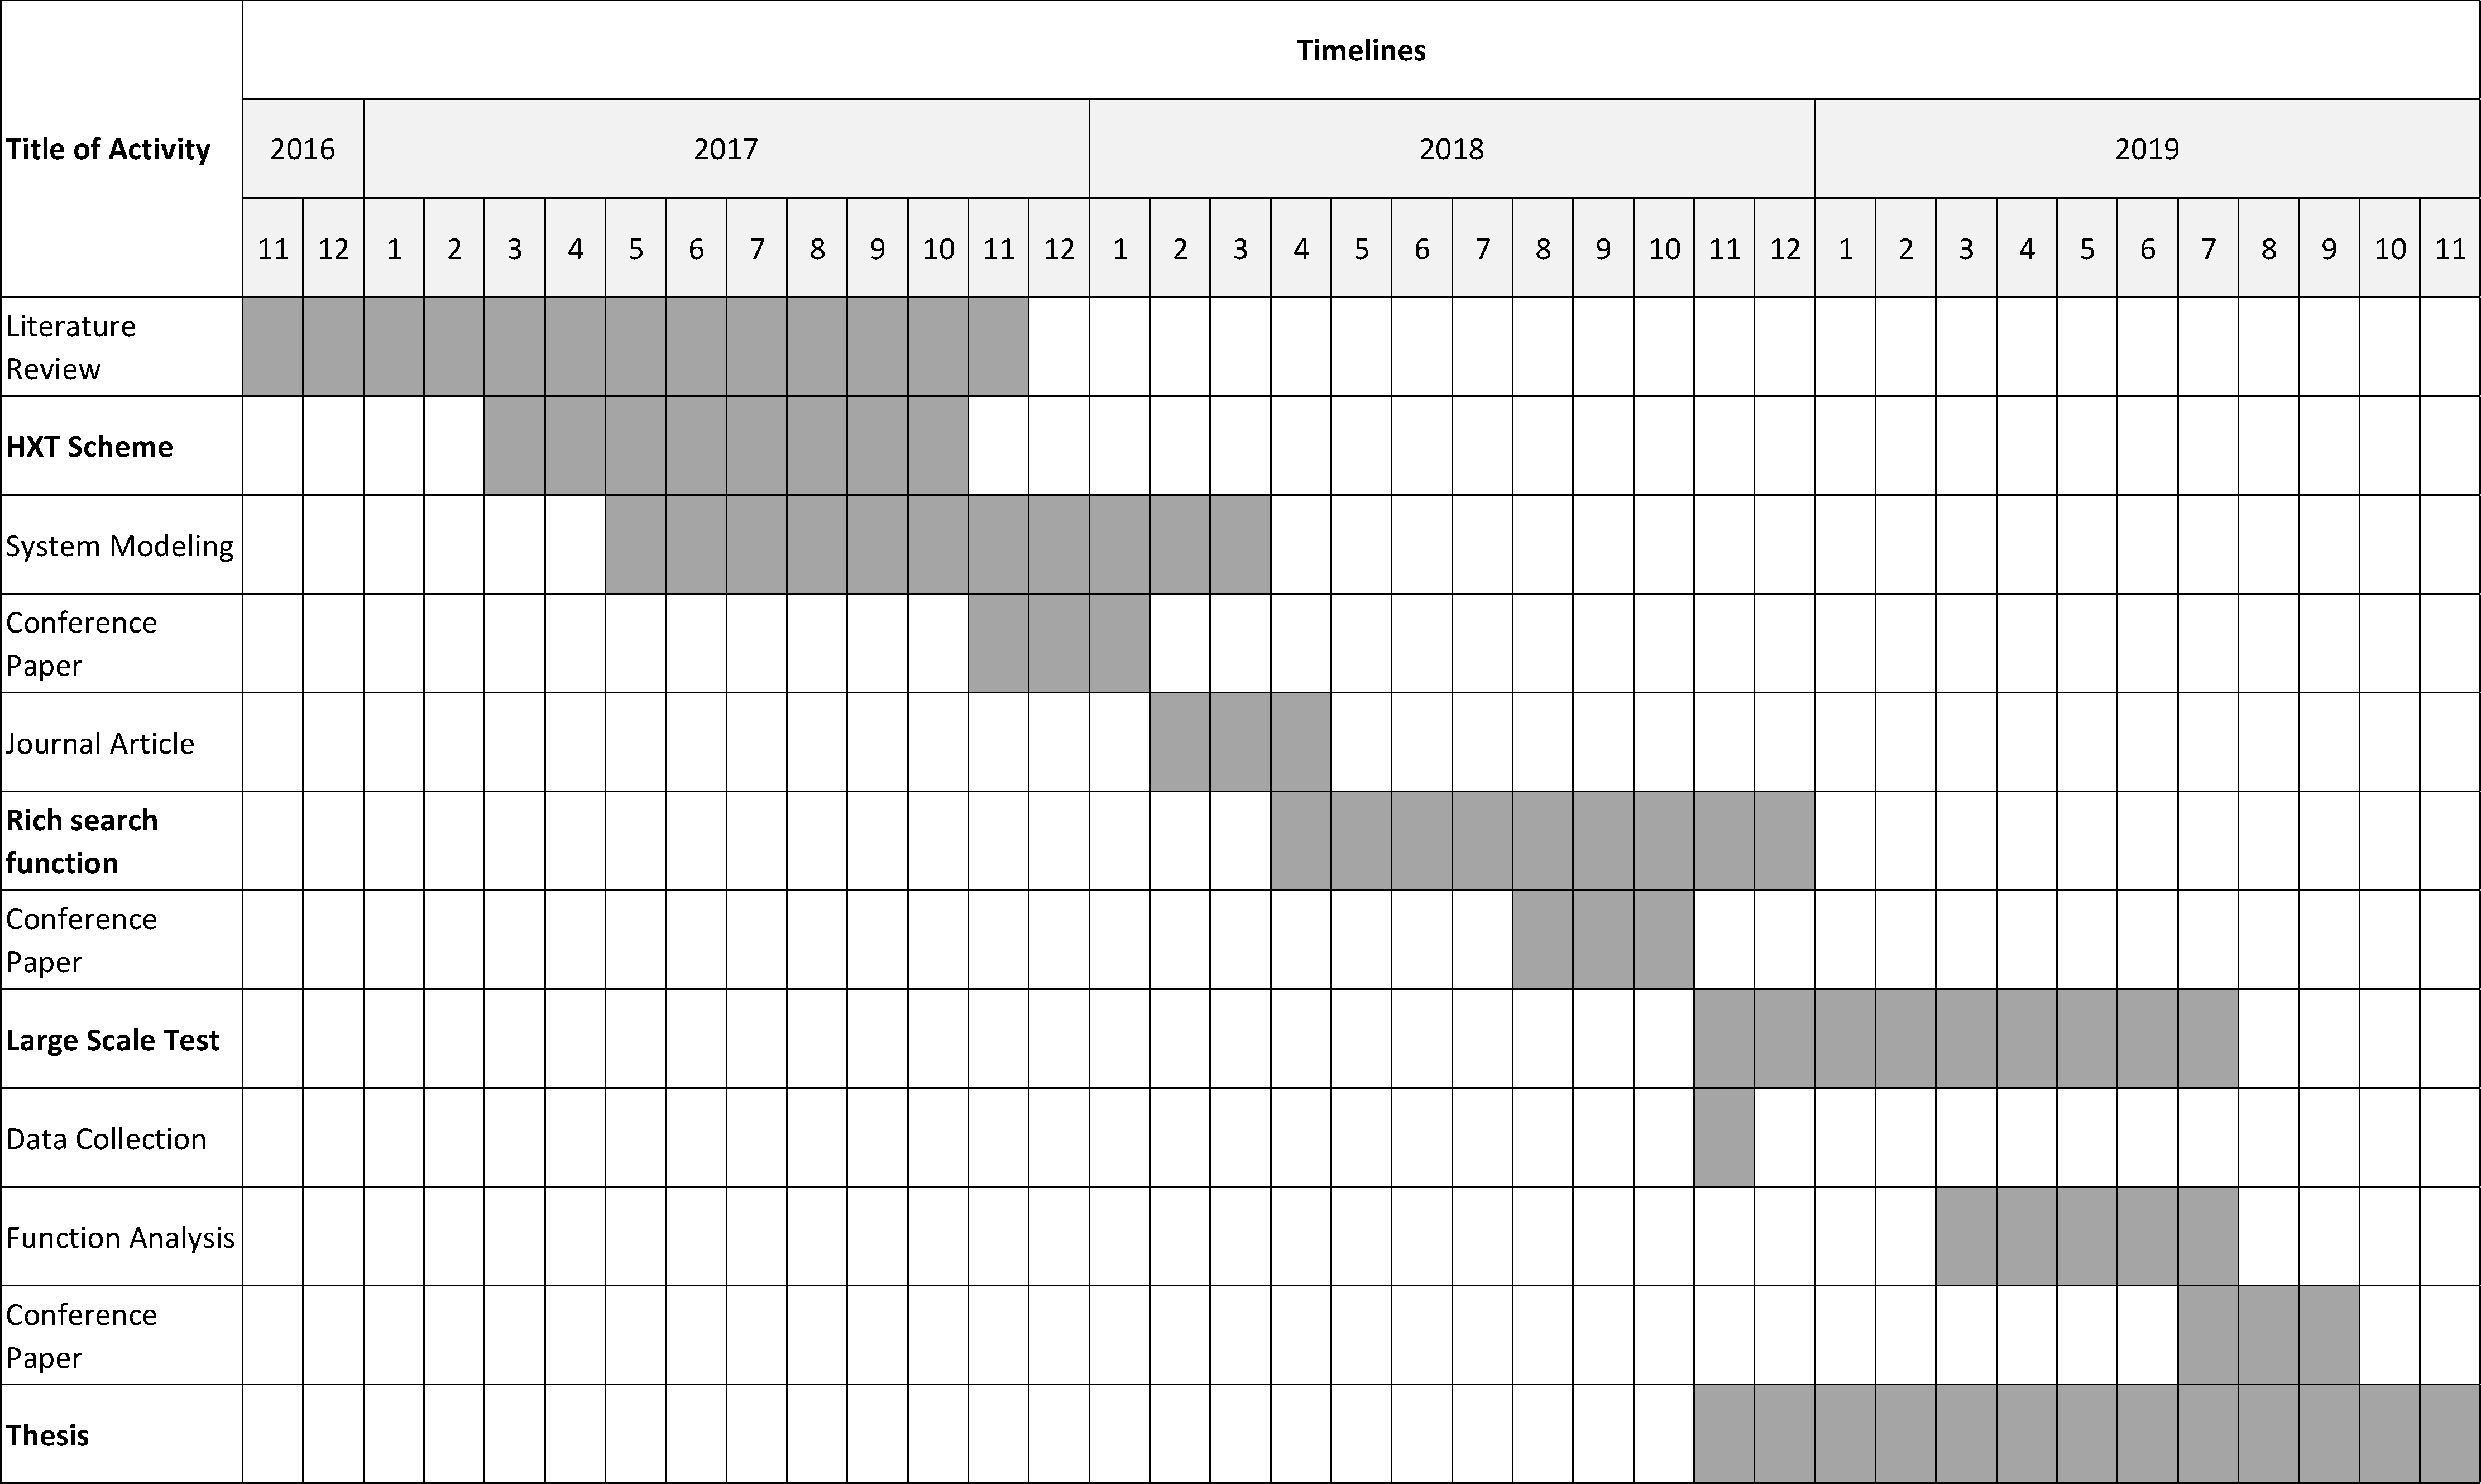
\includegraphics[width=\textwidth]{timeline.pdf}
\end{figure}
